\chapter{绪论}

\section{研究背景及意义}

\subsubsection{选题背景}

预训练模型是已经用广泛的样本训练过的模型。它已经在一个大型数据集上针对特定任务进行了训练。
% 
这个数据集可以是多种形式的,例如图像、文本或音频等。预训练模型的训练过程会产生一种通用的特征表示,这些特征可以被用来执行类似任务的新数据。
% 
从头开始训练一个深度学习模型可能需要花费数周或数月的时间,特别是在缺乏大量数据集的情况下(如BERT~\ucite{devlin2018bert}, GPT-3~\ucite{brown2020language})。
% 
在像ImageNet这样的大型数据集上训练神经网络,该数据集包含1000个类别的1400多万张图片,在这样的数据集上重新训练这样的模型是一种很大的开销。
% 
使用预训练模型可以作为模型的起点,这意味着,当为一个新任务微调预训练的模型时,我们不必从随机权重开始。
% 
而是可以使用预训练的权重作为初始化,然后只训练后面的特定于新任务的层。这需要更少的数据和训练时间。
% 
这可以节省大量的时间和精力。此外预训练模型有其他方面的优势。
% 
它们可以将知识从一般领域转移到特定领域。神经网络的浅层倾向于学习一般的特征,如边缘和形状,而后深则学习更具体的特征。
% 
因此,在一般图像上训练的预训练模型可以提供一般的低层次特征,然后你只需要为你的具体任务重新训练后面的层。这就是所谓的迁移学习。
% 
近年来,学术界和工业界都对开发精度更高,参数量更大的预训练模型感兴趣,因为采用较大的模型会带来更高的准确性。
% 
如图\ref{fig-dl}所示,近年机器学习模型参数量近几年呈现爆炸式增长。远远超出了常用GPU的显存限制(通常只有40-80GB,如Nvidia A100\ucite{nvidia_a100}),这也对我们如何快速,高效的训练模型提出了全新的挑战。

\begin{figure}[t]
\centering
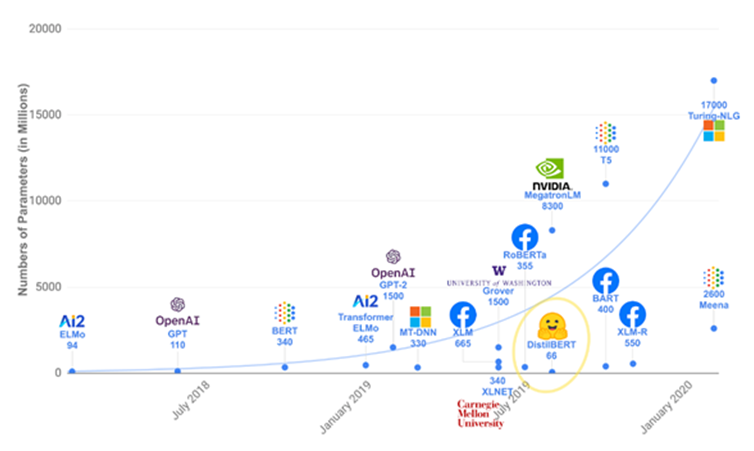
\includegraphics[width=0.7\linewidth]{fig1.png}
\caption{深度学习模型参数显著增长}
\label{fig-dl}
\end{figure}


研究人员表明,较大的模型会带来更高的准确性。
% 
从过去几年深度神经网络 (DNN) 驱动的机器学习技术的快速发展来看,研究者们发现加入更多 DNN 模型参数是最直接但不太复杂的方法之一提高 ML 算法的性能\ucite{kaplan2020scaling}。
% 
然而,DNN 模型容量通常受到计算资源和能源成本的限制\ucite{sharir2020cost}。
% 
根本原因是 DNN 的密集架构,其中计算成本通常与参数数量成线性比例。
% 
为了解决这种问题,混合专家 (MoE)~\ucite{lepikhin2020gshard} 在 DNN 中被广泛使用,它通过使用多个并行子模型(混合专家)引入了稀疏架构,其中每个输入经过门网络,动态选择并转发给少数专家处理。
% 
专家混合似乎有望将模型扩展到极端尺寸。
% 
如图\ref{fig-moe-training} 所示,与直接将小模型缩放为大密集模型不同,MoE\ucite{lepikhin2020gshard} 模型由许多小模型组成,即专家。
% 
训练样本被送入不同的专家,由轻量级可训练门网络动态选择。
% 
在 MoE 中,由于稀疏激活专家,节省了大量额外的计算量,与传统的密集型DNN相比,可以显着增加同一时间段内训练的样本数,提高模型精度。MoE技术是如今将DNN扩展到万亿参数的流行方法之一。

%
MoE混合专家系统是一种稀疏模型,因此其训练过程不同于传统的密集型DNN模型。主要有以下三点挑战:

\begin{itemize}
    \item 
    \textbf{动态激活特性:}
    MoE模型的稀疏激活特性使得它在GPU集群分布式训练时与现有的静态并行策略不匹配。
    因为MoE模型的每个样本只会被激活一个专家(也就是一个子模型),而其他的专家则不会被激活。
    这导致静态并行策略无法充分利用计算资源,因为只有部分计算节点被激活,而其他节点则处于空闲状态。
    % 因此,需要采用动态并行策略来适应MoE模型的稀疏激活特性,以最大限度地利用计算资源。

    \item 
    \textbf{额外通信开销:}
    MoE模型引入了GPU集群节点间额外的All-to-All通信,这种通信方式需要在所有计算节点之间进行数据传输和同步,由于All-to-All通信是一种同步通信方式,因此它会严重影响训练速度和效率。
    但是这种通信方式在MoE模型中是必需的,因为它需要将每个计算节点计算得到的结果进行汇总和组合,以得到最终的预测结果。

    \item 
    \textbf{节点负载不均衡:}
    由于MoE模型中的Gating在训练过程中不断变化,因此数据可能被分配到不同的专家上,导致负载分配不平衡的问题。
    如果某些专家的负载过高,而其他专家的负载过低,就会导致训练时间的延长和模型性能的下降。
    因此,需要根据每个专家的激活情况和计算负载进行动态的数据分配和负载均衡,以确保每个专家的计算负载均衡,并最大限度地利用计算资源。


\end{itemize}

现有的分布式训练框架\ucite{pytorch,deepspeed}对于其稀疏性的结构没有很好的支持,因此本次毕业设置拟设计一种更加高效的MoE训练框架,加速其分布式训练的过程,从而降低训练大规模的MoE模型架构的成本。

\begin{figure}[t!]
\vskip 2ex
\centering
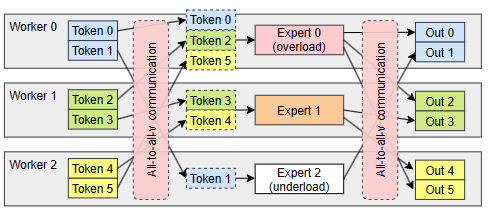
\includegraphics[width=0.69\linewidth]{fig6.png}
\caption{分布式MoE模型训练过程(图源\cite{he2021fastmoe})}
\label{fig-moe-training}
\end{figure}


\subsubsection{选题依据}
% 
随着人工智能技术的不断发展,MoE模型在各个领域都具有广泛的应用前景。它可以将多个不同的模型集成起来,以提高模型的性能和泛化能力。
% 
目前MoE模型在语音识别、自然语言处理、计算机视觉等领域都取得了很好的效果。
% 
因此,研究MoE模型的分布式训练和优化策略对于进一步提高模型的训练效率和性能具有重要意义。通过并行化和分布式计算等技术手段,可以加快MoE模型的训练过程,同时提高模型在大规模数据集上的效果。这将有助于应对深度学习任务和数据集日益复杂和庞大的挑战。
% 
此外,研究MoE模型的训练和优化策略不仅对于深度学习领域的研究具有重要意义,还能为各个领域的应用提供更高效和精确的解决方案。通过将多个专家的知识和能力结合起来,MoE模型能够更好地应对现实世界中的复杂问题,并提供更加准确和可靠的预测结果。
% 
因此,对MoE模型的分布式训练和优化策略进行深入研究,还能够在各个应用领域中取得更大的突破,为人工智能技术的进步做出重要贡献。

\section{深度学习训练系统及优化方法概述}
在本节中,我们从算法的角度演示了如何减少分布式DNN训练中的通信开销。算法优化包括减少通信轮次和通信量,以及增加计算-通信重叠率。这些优化与底层网络兼容,其中大多数可以在各种网络基础设施和协议之上运行。

\subsection{分布式深度学习训练系统概述}

分布式深度学习训练是一种将一个任务划分为较小的子任务并在多个处理器或设备上同时运行的技术\ucite{ben2019demystifying}。
% 
这种方法可以加快任务的执行速度,特别是当子任务可以在不同的处理器或设备上并行执行时。
% 
在分布式深度学习训练中,我们通过将训练数据和模型参数分布在多个处理器或设备上,然后在多个GPU上同时执行子任务来提高训练速度。
% 
这使我们能够突破单个GPU的内存限制,训练出比单个处理器或设备上所能训练的更大的深度学习模型。
% 
通过将训练过程在多个GPU上并行化,我们有效地增加了可用于训练模型的计算能力。每个GPU在训练数据的一个子集和模型参数的一部分上工作。然后通过汇总各个GPU的结果来建立整体模型。
% 
随着深度学习模型的规模和复杂性不断增加,分布式训练的好处变得更加明显。
% 
更大的神经网络需要更多的数据和计算来优化大量的权重和参数。
% 
通过利用多个GPU,我们可以扩大可用资源的规模,以满足这些大规模模型的需求。

目前,分布式深度学习训练中使用的并行性主要有三种类型:

\begin{itemize}
\item 
\textbf{数据并行性 (Data parallel)\ucite{ben2019demystifying}:}
在数据并行要求整个模型能够装入每个处理器或设备的内存中,这种方案将大规模的数据集分成多个小批次,分别在不同的处理器或设备上并行计算,以提高深度学习模型的训练速度和效率。
% 
在每个训练迭代或历时结束时,模型参数在所有处理器或设备上同步。
% 
更具体地说,每个处理器或设备在其训练数据部分的一批训练样本上工作。
% 
它在这个本地批次上执行前向和后向传播,以计算梯度并更新其模型副本中的权重和偏差。
% 
计算完成之后需要执行同步步骤,来自每个处理器或设备的模型参数被平均到一起(太频繁的同步会因为通信开销而降低训练速度,而太不频繁的同步则会导致独立的模型副本之间出现分歧)。
% 
通过数据并行和模型参数的定期同步,训练数据和计算可以有效地分布在多个处理器或设备上,以加快深度学习模型的训练。
% 
总的来说,数据并行难度相对较低,只需要并行化已有代码,但是其额外的通信开销随着GPU数量增加而增加,大规模训练性能较差。

Horovod\ucite{sergeev2018horovod}和Pytorchddp\ucite{li2020pytorch}是两个通常采用的数据并行训练系统,可使用All-Reduce同步梯度。 Byteps\ucite{peng2019generic}统一了全减少和参数服务器,并利用数据中心簇中的异质资源。 

\begin{figure}[t!]
    \vskip 2ex
    \centering
    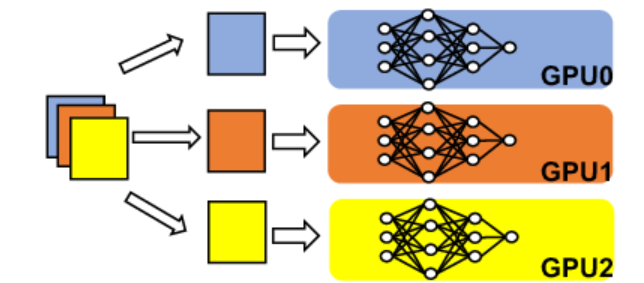
\includegraphics[width=0.7\linewidth]{figures/dataparallel.png}
    \caption{分布式训练-数据并行}
    \label{fig-data-parallel}
    \end{figure}

\item
\textbf{模型并行性 (Model parallel)\ucite{shazeer2018mesh}:}
模型并行可用于训练太大而无法放入单个处理器或设备的内存中的模型,但是需要处理器或设备之间进行更多通信模型的参数分割到多个GPU卡或服务器上训练。
% 
这种方法将复杂的深度学习模型分割成独立的子模型,并分配到多张GPU卡或服务器上,从而减少单个设备的计算负担。
% 
在每张GPU计算完成对应部分之后,需要将中间的激活值通过网络传输(NCCL\ucite{nccl})的方式发送给其他GPU参与后续阶段参与计算。
% 
使用模型并行需要对模型进行重构以分割参数,因此相应的并行度比较高。
% 
这种方式可以利用更多的计算资源来加速非常大模型的训练,但是参数分割和同步亦需要投入额外工作并存在较高的通信开销。
% 
总的来说,模型并行适合那些模块化清晰且参数易于分割的深度学习模型,并且可以更好地随处理器数量线性缩放。

\begin{figure}[h!]
    \vskip 2ex
    \centering
    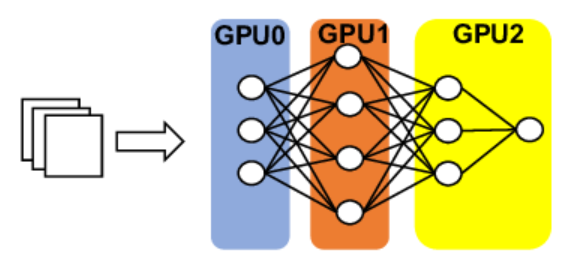
\includegraphics[width=0.7\linewidth]{figures/modelparallel.png}
    \caption{分布式训练-模型并行}
    \label{fig-model-parallel}
    \end{figure}

\item
\textbf{流水线并行 (Pipeline parallel)\ucite{huang2019gpipe}:}
流水线并行是一种通过将深度学习模型划分为多个独立阶段,并行执行不同阶段来加速训练模型的技术。具体操作包括:
% 
首先将模型分割成多个连续的阶段,如Embedding层、卷积层、池化层等
% 
并将一个Batch的数据划分为多个Macro-Batch分配给不同的阶段进行计算。
% 
当一个Macro-Batch通过一个阶段后,将结果传递给下个阶段,直至所有的Macro-batch通过流水线。
% 
不同阶段的计算可以同时执行,形成 computaional pipeline。
% 
整个Batch全部通过后,损失函数和梯度计算在最后一个阶段完成。
% 
流水线并行适用于很大的模型,超出单个GPU容量。它可以利用多个GPU来加速训练。
% 
流水线并行的优点是可以扩展到多个GPU来利用更多计算资源,利用计算资源更有效率。
% 
但是它主要挑战是需要更严格的同步不同阶段的计算,部分阶段可能存在空转,需要通过调整Macro-Batch大小来缓解。
% 
通常模型并行与流水线并行可能一起使用,以更好的平衡流水线并行中各个阶段的计算负载与数据通信开销。

\begin{figure}[t!]
    \vskip 2ex
    \centering
    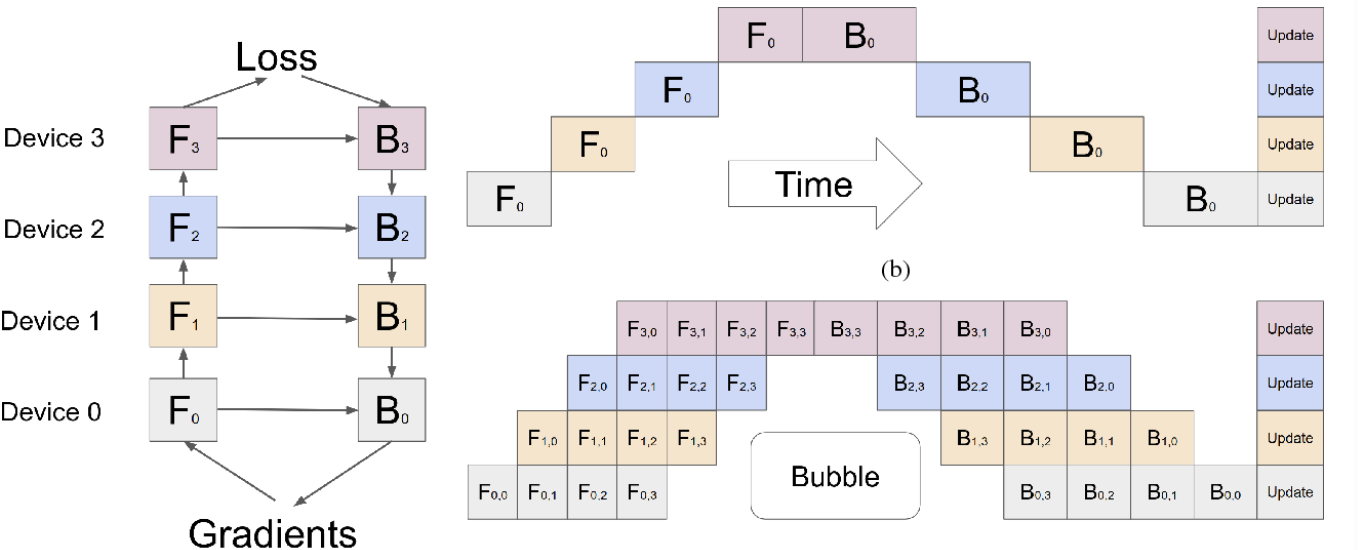
\includegraphics[width=0.7\linewidth]{figures/pipelineparallel.png}
    \caption{分布式训练-流水线并行(图源\cite{huang2019gpipe})}
    \label{fig-pipeline-parallel}
    \end{figure}

\item \textbf{自动并行(auto parallelism search)\ucite{zheng2022alpa}} 最近,研究者们提出了自动化寻找并行的策略的方式,即在深度学习分布式训练中,自动化并行通常指的是在给定GPU集群拓扑的情况下,通过自动化方法来选择和配置数据/模型/流水线并行方案。首先,自动化寻找并行策略的方式需要考虑许多因素,例如GPU数量、网络拓扑结构、数据集大小、模型结构和超参数等。这些因素之间的相互作用非常复杂,因此需要使用高级算法来解决优化问题。然而,这种算法的计算复杂度非常高,需要大量的计算资源和时间。
其次,自动化并行还需要考虑不同的并行方案之间的竞争和冲突。例如,多个GPU同时访问同一数据集可能会导致争用和延迟,从而影响训练的速度和质量。因此,需要使用先进的调度算法来解决这些问题。
最后,自动化并行的方式还需要考虑可扩展性和通用性。不同的深度学习任务可能需要不同的并行方案,因此需要使用通用的方法来解决这些问题。此外,随着GPU集群规模的增加,自动化并行的方式需要支持更大规模的计算,因此需要具有高度的可扩展性。
\end{itemize}

并行训练模型时,我们需要通过合理的任务划分和调度来优化深度学习训练的效率和可扩展性,并根据深度学习模型本身的特点和可用的硬件资源选择最佳的并行方案。从而在保证模型精度的同时,实现训练速度提升,支持更大规模的训练,以及提高可靠性和容错性。
% 
这种方式可以更充分地利用计算资源,提高深度学习模型的训练效率和可扩展性,从而适应越来越复杂和庞大的深度学习任务和数据集的需求。



\subsection{算法层面训练优化}
当使用SGD训练深度神经网络时,整个训练过程通常由多个时期和迭代组成。关于并行化,节点通常在每次迭代结束时交换数据。减少通信开销的一种直观方法是减少数据交换或通信轮次的数量。节点的轮次与批量大小和通信周期有关。更大的批量和更长的通信周期都可以减少数据交换轮次。

\noindent \textbf{调整批量大小:}
批量大小是一个重要的超参数,用于控制节点在每次迭代中读取的数据量。较大的批量通常比较小的批量更接近输入数据的分布,并且在梯度估计中引入较少的方差。然而,使用大批量处理数据会导致更长的处理时间和较少的模型参数更新。这一发现主要是由于批量大小、迭代次数和训练数据大小之间的关系。

大批量的使用会导致迭代次数的减少,从而减少了参数更新的频率。在具有数据并行方案的分布式训练环境中,批大小是每个节点的本地批大小的总和。在传统的分布式深度学习中,节点在每次迭代结束时交换梯度和模型参数。因为参数仅取决于深度神经网络(DNN)本身,单次迭代传递的消息大小保持不变,即使改变了批量大小,消息的形状和大小也不会改变。因此,增加批量大小可以减少迭代次数和通信轮次\ucite{Ouyangjpdc21}。

然而,在实践中,通过直接使用巨大的批量进行并行随机梯度下降(SGD)训练时,与训练小批量相比,可能会出现泛化能力下降的问题。这是因为较大的批量可能会导致模型过度依赖于批量内部的统计特性,而忽略了数据集的整体分布。较大的批量也可能会使模型更难以逃离局部极小值,从而限制了其学习能力\ucite{you2019fast}。

因此,在确定批量大小时需要进行权衡。较小的批量可以提供更多的参数更新和更快的收敛速度,但估计的梯度可能会受到较大的方差影响。较大的批量可以减少方差,但会导致更少的参数更新和更长的训练时间,并可能对模型的泛化能力产生负面影响。选择合适的批量大小需要综合考虑数据集的规模、计算资源、训练时间和模型的泛化需求。

因此,在实际应用中,可以通过调整批量大小并进行实验评估来确定最佳的超参数配置,以获得更好的模型性能和泛化能力。

\noindent \textbf{周期性通信:}
当使用传统的分布式随机梯度下降(SGD)训练深度神经网络(DNN)时,通信通常在每次迭代的末尾进行。然而,许多研究建议减少梯度和参数的交换频率,以降低通信开销并提高训练效率。

在梯度同步的过程中,每个局部节点上训练的模型参数以一定周期 r 进行平均梯度。传统的梯度同步通常在每轮训练结束时进行,即 r=1。然而,一些研究工作~\ucite{stich2019local}提出将梯度平均的周期设置为 1 < r < T,其中 T 是总的训练轮数。通过将梯度平均的周期设置为介于 1 和 T 之间的值,可以减少模型训练过程中的通信开销。

通过减少梯度和参数的交换频率,可以降低通信带宽的要求,减少网络传输的延迟,并提高分布式训练的效率。通过在一定周期内对梯度进行平均,可以减少通信的次数,从而减少训练过程中的通信开销。

然而,选择合适的梯度平均周期 r 也需要进行权衡。较大的 r 值可以降低通信频率,但可能会导致模型更新的延迟和不准确性。较小的 r 值可以提高梯度的准确性,但会增加通信的次数和开销。因此,需要根据具体的应用场景和系统约束来选择适当的梯度平均周期。

综上所述,通过调整梯度平均的周期,可以在分布式训练中减少通信开销,提高训练效率,并在一定程度上平衡模型更新的准确性和延迟。这些技术的应用可以帮助加快深度神经网络的训练速度,提高分布式训练的可扩展性和性能。



\noindent \textbf{模型梯度压缩:}
% 
模型梯度压缩是一种用于减少分布式深度学习通信量的技术。在分布式深度学习中,多个计算节点共同训练一个模型,这些节点需要在每个训练步骤中共享模型参数的更新。这种通信需要传输大量的数据,通常会成为分布式训练的瓶颈\ucite{cheng2017survey}。

模型梯度压缩通过减少传输的数据量来缓解这种问题。具体而言,该技术通过对模型梯度进行压缩来减少通信量。压缩的方式可以是量化、稀疏化、低秩分解等。

量化是一种常见的压缩方法,它将浮点数转换为较小的整数或定点数。这样可以大大减少传输的数据量,但也会导致精度损失\ucite{zhou2018adaptive}。为了减轻精度损失,研究人员开发了一些基于量化的方法,如误差反向传播(Error Feedback Backpropagation,EFB)\ucite{jacob2018quantization}和Top-k\ucite{pham2018efficient}选择。

稀疏化是另一种常见的压缩方法,它将模型梯度中的某些元素设置为零。这样可以减少传输的数据量,但也会导致一些信息的丢失。为了保留尽可能多的信息,研究人员开发了一些基于稀疏化的方法,如稀疏梯度蒸馏, 模型剪枝选择\ucite{liu2018rethinking}。

低秩分解是一种将原始矩阵分解为多个低秩矩阵的方法,从而减少矩阵的大小。这种方法已经被应用于分布式深度学习中,例如矩阵分解(Matrix Factorization,MF)和低秩近似\ucite{hu2021lora}.

\subsection{系统层面训练优化}

\noindent \textbf{加速DNN模型训练:}
通信优化在分布式深度学习训练系统中起着至关重要的作用,它可以减少通信开销、降低训练时间,并提高系统的可扩展性。下面介绍几种常见的通信优化方式:
\begin{itemize}
    \item 使用RDMA\ucite{gdr}或NCCL\ucite{nccl}来加速单个消息:RDMA(Remote Direct Memory Access)和NCCL(NVIDIA Collective Communications Library)是一些常用的通信优化技术。RDMA技术可以直接在计算节点之间进行内存数据传输,绕过CPU的参与,从而减少通信的延迟。NCCL是一种专门为GPU集群设计的高性能通信库,它能够充分利用GPU的计算能力来加速通信操作。
    \item 压缩数据传输,例如梯度量化\ucite{pham2018efficient}和稀疏参数同步\ucite{fei2021efficient}:梯度量化和稀疏参数同步是常用的数据传输压缩技术。梯度量化将浮点数梯度转换为较小的整数或定点数,从而减少传输的数据量。稀疏参数同步则将模型参数中的部分元素设置为零,只传输非零元素的索引和值,从而减少传输的数据量。
    \item 优化通信方法,例如对于PS和不同的All-reduce算法研究者们根据架构信息提出了不同的优化加速方式\ucite{daily2018gossipgrad}\ucite{peng2019generic}。例如,对于参数服务器(Parameter Server)可以根据深度学习模型的特点,为每一层设计不同的通信方式,调整同步策略,以减少通信开销。而All-reduce中可以采用异步通信中维持全局模型一致性的方法优化通信,它可以减少通信的同步开销。
    \item 通过使用流控制(flow control)\ucite{mai2015optimizing}或Coflow调度\ucite{chowdhury2014efficient},最大程度地减少网络流量完成时间:流控制和Coflow调度是一些优化网络流量的技术。流控制通过调整发送和接收的速率来避免网络拥塞,减少数据传输的延迟。Coflow计划则将相关的数据流组合在一起,进行优化调度,以最大程度地减少数据传输的时间。
\end{itemize}


\begin{figure}[t!]
    \vskip 2ex
    \centering
    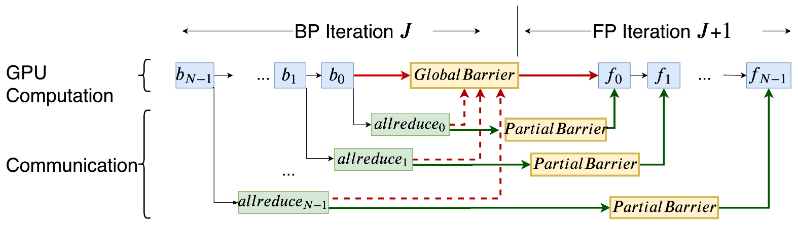
\includegraphics[width=0.7\linewidth]{figures/bytescheduler.png}
    \caption{通信计算在Forward/Backward过程中重叠(图源\ucite{peng2019generic})}
    \label{fig-bytescheduler}
\end{figure}


\noindent \textbf{将通信与计算重叠:}
大多数深度神经网络(DNN)框架,如Tensorflow、PyTorch、MXNet和Posei-Don [39],都支持使用反向传播时的重叠通信。其中,P3\ucite{jayarajan2019priority}进一步探索了如何通过对MXNet的参数服务器体系结构进行图层分区和调度来实现正向传播的重叠。类似地,TIC-TAC\ucite{hashemi2019tictac}提出了一个类似的思想,但其基于Tensorflow的参数服务器(PS)的训练速度较慢(小于20\%)。Bytescheduler\ucite{peng2019generic}结合模型具体特征调整训练方式,尽可能最大化通信与计算的重叠,从而提升计算速度。并且,Bytescheduler在多个DNN框架中,多种通信方式(RDMA/TCP/IP)都是通用的。作者对已有调度算法进行了分析,克服了它们的缺点,例如不适应系统开销和全局同步的限制,并实现了更高的加速度。Bytescheduler提供了在多个DNN框架中使用的通用优化策略,能够克服现有方法的缺点。该方法充分考虑了系统开销以及全局同步所带来的限制,并采用了有效的调度算法。Bytescheduler实现了更高的训练加速度,为深度学习研究和应用提供了重要的贡献。
SYNDICATE\ucite{mahajan2023better}在bytescheduler的基础上更进一步,将网络拓扑与模型架构联合考虑从而实现通信-计算,通信-通信的重叠,从而极大程度的提高了模型训练速度。SYNDICATE设计了一种有关通信原语代数表示,将原本的通信原语分解为很小的motifs,以motifs为力度调度,从而实现了更加细粒度的调度策略,提升了模型训练系统吞吐量。

\noindent \textbf{内存优化:}
Zero Redundancy Optimizer(零冗余优化器)\ucite{rajbhandari2020zero,ren2021zero}是一种用于深度神经网络训练的优化方法,旨在减少参数服务器(PS)之间的通信冗余,从而提高训练效率。该方法的核心思想是通过在每个参数服务器上只存储和更新模型的一部分参数来减少通信开销。

传统的分布式训练中,每个参数服务器都存储完整的模型参数,并在每个训练步骤中进行同步通信以更新参数。这种全局同步的方式会导致较高的通信开销,尤其是当模型规模较大时。Zero Redundancy Optimizer则采用了一种新的策略,将模型参数分割为多个部分,并将每个部分分配给不同的参数服务器。这样,每个参数服务器只需要存储和处理分配给它的参数部分,而不再需要与其他服务器进行通信。这样,每个GPU只需要存储和处理自己所负责的参数部分,而不需要存储整个模型参数。通过减少每个GPU显存中所存储的参数量,从而有效地降低了显存的使用。

Zero Redundancy Optimizer的关键优势在于减少了参数服务器之间的通信量,从而显著降低了通信开销,提高了训练效率。它允许每个参数服务器独立地更新自己所负责的参数部分,而不需要与其他服务器同步。这种方式可以充分利用计算资源,加速模型训练过程。

然而,Zero Redundancy Optimizer也引入了一些挑战和限制。首先,由于参数被分割到不同的服务器上,模型更新可能不再是全局同步的,这可能导致一些收敛性问题。因此,需要仔细设计合适的同步策略,以确保模型能够收敛到良好的结果。其次,参数分割的方式需要根据具体的网络结构和训练需求进行设计,这对于大规模模型的优化来说可能是一项复杂的任务。

\section{国内外研究现状}

\subsection{MoE训练系统}
随着MoE训练范式的普及,许多科研机构和企业都开源了MoE训练框架和系统。 
% 
DeepSpeed-MoE 利用多种分布式并行方法结合 MoE 并行性,包括数据并行、张量切片\ucite{shoeybi2019megatron}、Zero内存优化\ucite{rajbhandari2020zero}来训练更大的模型。至于 MoE 的推理,DeepSpeed\ucite{rajbhandari2022deepspeed}设计了一种名为 PR-MoE 的新型稀疏激活模型和模型压缩技术来减小 MoE 模型的大小,以及一种有效的通信方法来优化延迟。 
% 
FastMoE\ucite{he2021fastmoe} 是一个分布式 MoE 训练系统,它提供了一个分层接口和简单的机构,说明如何基于数据并行性和张量切片并行性使用 Megatron-LM\ucite{shoeybi2019megatron} 和 Transformer-XL\ucite{dai2019transformer}。
% 
与 DeepSpeed 的实施不同,FastMoE 使用复杂的优化方法来减少网络流量。
% 
Fairseq-MoE\ucite{ott2019fairseq}  是一个序列建模框架,用于训练用于摘要、翻译和语言建模的自定义模型。
% 
而 Tutel\ucite{hwang2022tutel} 在通信和计算方面进一步优化了 Fairseq 系统,其性能提升了约 40\%。
Tutel 中的优化已集成到 DeepSpeed 中,以促进 MoE 模型训练。

\subsection{MoE数据分派策略}
MoE的核心问题之一是如何设计gating策略,即如何根据输入分配不同的专家网络。不同的gating策略会影响模型的性能、稀疏性、均衡性和公平性。
\begin{itemize}
    \item \textbf{Softmax gating}\ucite{he2021fastmoe}:这是最简单的一种gating策略,它使用一个softmax层来为每个输入分配一个概率分布,表示每个专家网络的权重。这种方法可以看作是多个专家网络合作来产生输出,但是也会导致所有的专家网络都被激活,从而增加计算量和内存消耗。
    \item \textbf{Top-k gating}\ucite{hwang2022tutel}:这种gating策略只选择概率最高的k个专家网络来处理输入,其他的专家网络则被忽略。这种方法可以实现稀疏性,即只有少数的专家网络被激活,从而节省计算量和内存消耗。但是这种方法也会带来一些问题,比如如何确定k的值,以及如何保证每个专家网络都能被充分利用。
    \item \textbf{Noisy softmax gating}\ucite{xu2022survey}:这种gating策略在softmax gating的基础上增加了一个可学习的噪声权重,用来提高不同专家网络的gating均衡性。这种方法可以防止某些专家网络被过度使用或者被忽略,从而提高模型的公平性和泛化能力。
    \item \textbf{Hierarchical softmax gating}\ucite{xu2022survey}:这种gating策略将多个专家网络组织成一个层次结构,每一层都有一个softmax gating来决定下一层的激活。这种方法可以减少softmax gating的计算复杂度,从而提高模型的效率。
    \item \textbf{Hash layer}\ucite{roller2021hash}:这种gating策略使用哈希函数来为每个输入分配一个或多个专家网络,而不需要学习任何参数或者使用额外的损失函数。这种方法可以实现极高的稀疏性和效率,同时保持或者提升模型的性能。
    \item \textbf{Topology-aware gating}\ucite{chen2022ta}: TA-MoE中提出了一种拓扑感知的路由策略,它能够根据网络拓扑的变化动态地调整MoE的数据分派的调度策略。通过基于通信建模的方法,TA-MoE将调度问题抽象为一个优化目标,并得到了适用于不同拓扑结构的近似调度模式。他们设计了一种拓扑感知辅助损失函数,它可以自适应地根据底层拓扑调整数据分派策略,而不会牺牲模型的准确性。
\end{itemize}



\section{研究目标}

本课题针对MoE模型带来以上挑战,拟分析现有的MoE模型分布式训练系统存在的缺陷,并设计一套全新的MoE模型训练系统。

MoE模型在分布式训练中面临几个挑战。首先,MoE模型的稀疏激活特性与现有的静态并行策略不匹配,导致计算资源无法充分利用。其次,MoE模型引入了全局所有GPU之间同步的All-to-All通信,严重影响训练速度和效率。最后,由于Gating策略的动态变化,节点负载可能不均衡,导致训练时间延长和模型性能下降。因此,需要采用动态并行策略、优化通信开销和实现负载均衡,以克服这些挑战,提高MoE模型的训练效率和性能。

如图\ref{fig-overview}所示,我们提出了一种全新的MoE训练系统,通过在算法层面(gating policy)和系统层面(Expert placement scheduler)提出创新的训练解决方案,旨在克服MoE模型训练过程中的瓶颈,并更好地适应复杂而庞大的深度学习任务需求。
\begin{figure}[h!]
    \vskip 2ex
    \centering
    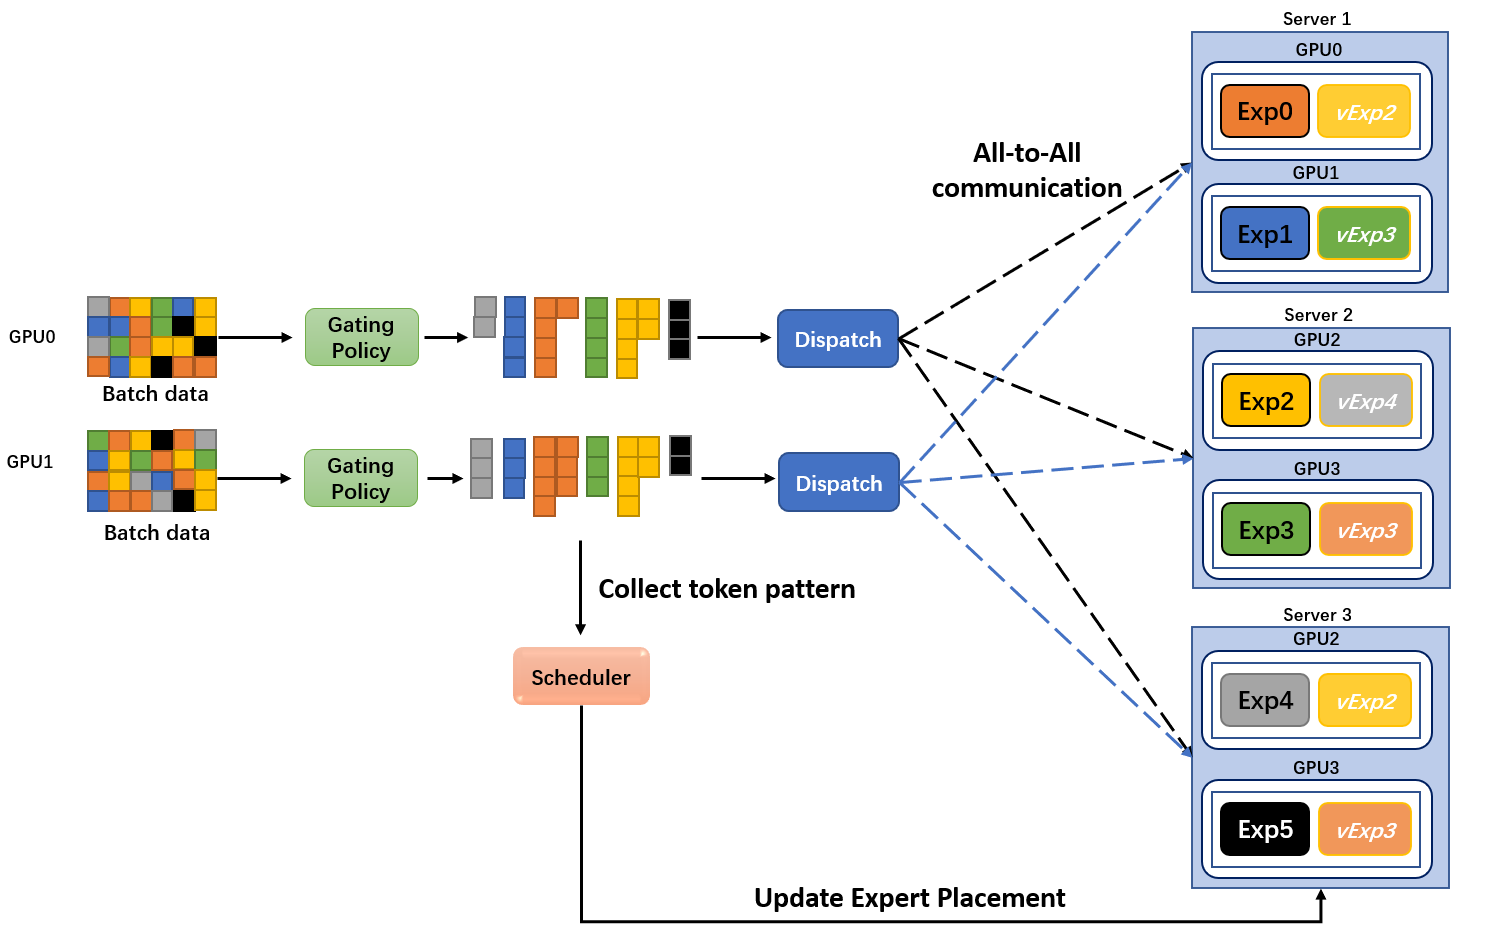
\includegraphics[width=0.99\linewidth]{figures/fig7.png}
    \caption{设计的MoE训练框架}
    \label{fig-overview}
    \end{figure}


我们的训练系统综合考虑了多个因素,包括任务特性、训练系统的拓扑结构、训练数据的分布以及每个专家的能力。通过算法与系统的协同设计,我们致力于实现能够动态优化专家的分布式并行策略,使每个专家都能够发挥最大潜力,并在整个系统中平衡负载和资源利用率。

在算法层面上,我们对MoE模型的数据分派关键部分,即gating策略,进行了改进。通过动态调整数据分派策略,我们实现了更快的收敛速度,并同时控制了全局通信开销。我们采用了All-to-All通信原语中的unequal模式,进一步减少由填充(padding)引起的额外数据发送量,从而降低全局通信的成本。

同时,在系统层面上,我们提出了一种基于网络拓扑的自动负载均衡策略。我们根据训练系统实际的网络拓扑结构,研究了不同拓扑结构下的数据传输和通信开销,并针对性地设计了一种优化策略。通过充分利用数据的局部性和专家之间的并行计算能力,我们能够减少通信开销,提高整体训练效率。
% 
我们的设计在offline的过程中,首先根据系统的网络拓扑结构,分析训练系统中任意两点进行通信操作的开销,并建立数学模型。
% 
在online过程中,我们设计了一种调度器(Expert placement scheduler),它能够收集并监测每一个MoE层中所有专家的任务负载。
% 
当检测到专家的负载发生一定变化时,调度器会根据当前负载情况和专家的放置情况,自动寻找最合适的专家并行放置策略,从而解决MoE模型在训练过程中由于负载动态变化而导致的训练效率低下的问题。
% 

这种全新的训练解决方案使得MoE模型能够更好地应对复杂和庞大的深度学习任务需求。通过优化算法和系统设计,我们能够充分发挥MoE模型的潜力,提高模型的准确性和泛化能力,为解决现实世界中的复杂问题提供有力工具。我们的研究对推动MoE技术的发展和应用具有重要意义,也对分布式训练系统的进一步发展起到推动作用。

\subsection{基于动态路由的数据分派策略}

\begin{figure}[h!]
\vskip 2ex
\centering
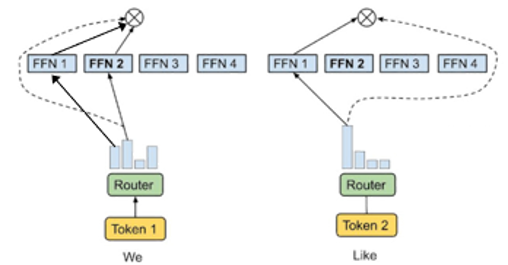
\includegraphics[width=0.5\linewidth]{figures/fig3.png}
\caption{传统的Top1和Top2 Gating策略}
\label{fig-top1_top2}
\end{figure}

如图\ref{fig-top1_top2}所示在传统的MoE模型中,采用固定的Top1和Top2 Gating策略,即将数据发送到分数最高(次高)的expert进行处理。
% 
然而,采用Top1 Gating时,由于只选择一个最高分数的expert,可能会错过其他有价值的信息,导致模型收敛速度较慢;
% 
而采用Top2 Gating时,虽然可以选择两个最高分数的expert,但每轮训练时间较长,因为需要进行两次All-to-All通信。
% 
因此我们能否将Top1和Top2 Gating策略结合起来,以一种动态的方式选择合适的数据分派策略,从而实现较快的收敛速度和较短的训练时间。
% 
一种简单的方法是,将每个数据按照Top1和Top2的分数进行排序,然后将它们分别分配给Top1和Top2的expert进行处理。
% 
这种方法可以利用Top1和Top2的优点,避免错过其他有价值的信息,同时减少通信开销,提高训练效率。

\subsection{基于网络拓扑的自动负载均衡策略}


\begin{figure}[t!]
\vskip 2ex
    \begin{minipage}[h]{0.48\linewidth}
        \centering
        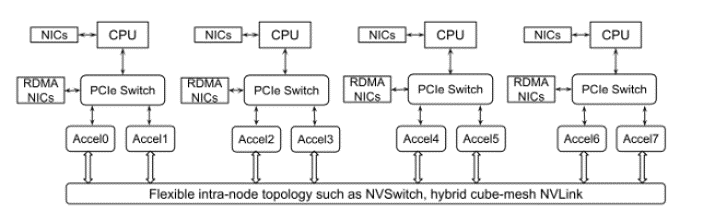
\includegraphics[width=1\linewidth]{figures/fig4.png}
        \caption{GPU集群内网络拓扑连接图(图源\cite{mahajan2023better})}
        \label{fig-kek-tree}
    \end{minipage}
    %
    \begin{minipage}[h]{0.48\linewidth}
        \centering
        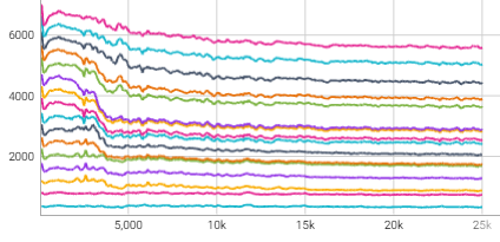
\includegraphics[width=0.8\linewidth]{figures/fig5.png}
        \caption{8层128专家的Transformer-XL\ucite{dai2019transformer}的MoE模型,第1层16个专家负载变化情况}
        \label{fig-transformer-xl}        
    \end{minipage}
\end{figure}

虽然基于 MoE 的算法开辟了一个巨大扩展模型参数量机会,但它也对训练系统带来了新的挑战,而这些挑战在之前的密集型DNN训练算法和系统中从未见过。根本原因是动态专家选择和灵活的 MoE 结构。具体来说,每个 MoE 层由一定数量的并行专家组成,这些专家分布在加速器(本工作中的 GPU)上,其中每个 GPU 根据智能门函数将每个输入数据分配给几个最适合的专家并取回相应的输出以将它们组合起来。这意味着每个专家的工作量基本上是不确定的,取决于输入数据和门函数。在图\ref{fig-transformer-xl}中,我们使用了一个8层的Transformer-xl MoE模型,分析了第1层16个专家负载变化情况。

我们发现,在MoE模型中,不同专家的负载在每次迭代中都会发生变化。
% 
这种现象是由于MoE的稀疏性动态数据分配所导致的,导致每个专家获取的数据不均匀,从而产生了负载不均衡的问题。
% 
这会导致一些节点或expert的负载过重,从而影响整个模型的训练速度和效果。因此,需要采取适当的负载均衡策略来缓解这个问题。
% 
此外在MoE模型中所有专家都需要从其他GPU上那里获得输入,这引入了GPU集群所有节点间额外的All-to-All通信,且All-to-All通信与后续计算是完全同步关系,并行较差。
% 
而GPU集群内部节点之间的网络带宽并不相同,节点通信效率存在差异。
% 
因而All-to-All通信也成为了大规模MoE训练中最耗时的操作之一。
% 
它通常实现为具有可变消息大小的同步 All-to-All 操作。考虑到动态特性的数据分派会导致计算和通信的严重不平衡,这样的方法会导致严重的开销。

因此,为了解决负载不均衡问题,需要采取一些适当的负载均衡策略,我们需要结合GPU集群内部节点之间的网络带宽不相同的情况,选择最佳的负载均衡策略,以提高整个模型的训练效率和性能。

\section{本文组织结构}

本文的组织结构如下:

本文的第二章是MoE训练过程的概述。
% 
该章主要介绍了MoE混合专家模型在分布式深度学习训练中的主要过程,分析了其正向反向传播的计算过程,并解释了为什么MoE模型与现有传统集中式训练系统的不匹配。

本文的第三章是基于动态路由的数据分派策略的设计方式。
%
该章首先分析了现有的数据分派策略的主要方式,并总结了现有设计的不足之处。进而更进一步,给出了我们设计的基于动态路由的数据分派策略具体的方案架构,包括方案的详细流程和性能分析。


本文的第四章为基于网络拓扑的自动负载均衡策略方案设计。
%
该章首先分析了现有GPU数据中心网络拓扑。并结合每个专家在训练过程的负载变化现象,建立模型寻找最佳的负载均衡方案设计。


本文的第五章为系统实现以及实验结果展示。
%
该章给出了整体的设计方案以及实验结果展示。

本文的第六章为总结与展望。
%
该章总结了本文的主要贡献,以及对未来工作的展望。


\section{本章小结}

本章首先对论文选题的背景和研究意义进行讨论,提出了稀疏混合专家MoE模型对于现有深度学习训练系统的挑战。
%
随后对国内外研究现状进行了简要的介绍。
最后我们介绍了本工作的研究内容和研究目标。我们分析了MoE模型在分布式训练系统中的挑战,并介绍了设计的全新MoE模型训练系统。该系统在算法层面和系统层面提出了创新的训练解决方案,旨在克服MoE模型训练过程中的瓶颈,并更好地适应复杂而庞大的深度学习任务需求。
\endinput